\chapter{Development and\\Implementation}
\label{cha:implementation}
\chapterquote{It's done, when it's done}{An English Phrase}

\section{Outline}
The sections in this chapter will describe the various stages of development and implementation of this Bachelor thesis' application. At first the basic idea of the layout and the individual views will be described and explained. To get an even better impression the early paper prototype will be shown. Afterwards a short description of the aspired time schedule for the development as well as the creation of the written elaboration is given.

The implementation of the basic layout which was displayed and explained with the help of the paper prototype, will be the first part describing the actual implementation process.
Second, the handling of the data to be visualized is explained. This covers the server based access as well as local storing and loading. 

After the preparations for the visualization have been set forth, the different views will be described. Starting with the explanation of the map view, it will be clarified how the loaded data is visualized. This is followed by the section focusing on the chart view. It explains how a library is used to draw pie charts and how the loaded data has to be prepared. The last section describes how the timeline was implemented. It covers, how one can draw its own views in Android and how to make use of gestures.
\newpage
\section{Paper Prototype}
\label{sec:paper_prototype}
The first step of the development process was the creation of a paper prototype. It was needed to demonstrate the idea and visual appearance of the project and application. Another advantage of the paper prototype is to be able to show the application to  different people and to get feedback without even writing one line of code. This provides the ability to eliminate possible false estimations  in the forefront of the application's implementation. False estimations may be the assumption of wrong needs of possible future users or the creation of an non intuitive layout. In the following the paper prototype will be shown and explained.

The\mnote{Basic layout} first idea was to split the screen into two parts, an option part and a view part. The left part should be the option part, occupying one sixth of the visible screen. It should always display the following, in appearing order listed, options.\\
In the top left a view selection containing three buttons  ordered vertically with titles ``Map-View'', ``Chart-View'' and ``Timeline'' are displayed. Taping one of those buttons causes a view switch to display the respective view.\\
Under the view selection a list of options should be visible. Those options vary from view to view but should always contain a button at the top of the list displaying the currently selected date. Tapping on this button causes a date-selection-window to pop up. Selecting a date leads to an update of the displayed view, now visualizing the respective data.
Other options will be explained together with their respective views.

When \mnote{Map-View} the application has been loaded, the user will be displayed the map view thus making it the application's start view. The view will display a map with a route, representing the user's visited locations. On start up the selected date will be the current day and therefor the draw route represents the user's latest movements. Tapping on the route should bring up a speech bubble which contains information about the tapped location. Those informations will be the time spend on that location, the used applications and possibly shot photos.\\
The \mnote{Map-View specific options} view provides two special options. The first option is represented by a check box and has the title ``Photos''. The option provides the ability to highlight those locations, where a photo was taken. The second option is called ``Apps''. It lets the user pick applications from a list and colors all parts of the route where those specified applications were used. Those options would provide a great tool to quickly get an overview over the position data of specific applications and actions. An actual image of the paper prototype for the map view can be found in figure \ref{img:mapview}.

The map view can mainly be used to answer the question ``Where was smartphone used?'', since the view focuses on visualize the map and traveled routes rather than displaying numbers and percentages.
\begin{figure}[h]
	\caption{Map-View}
	\label{img:mapview}
	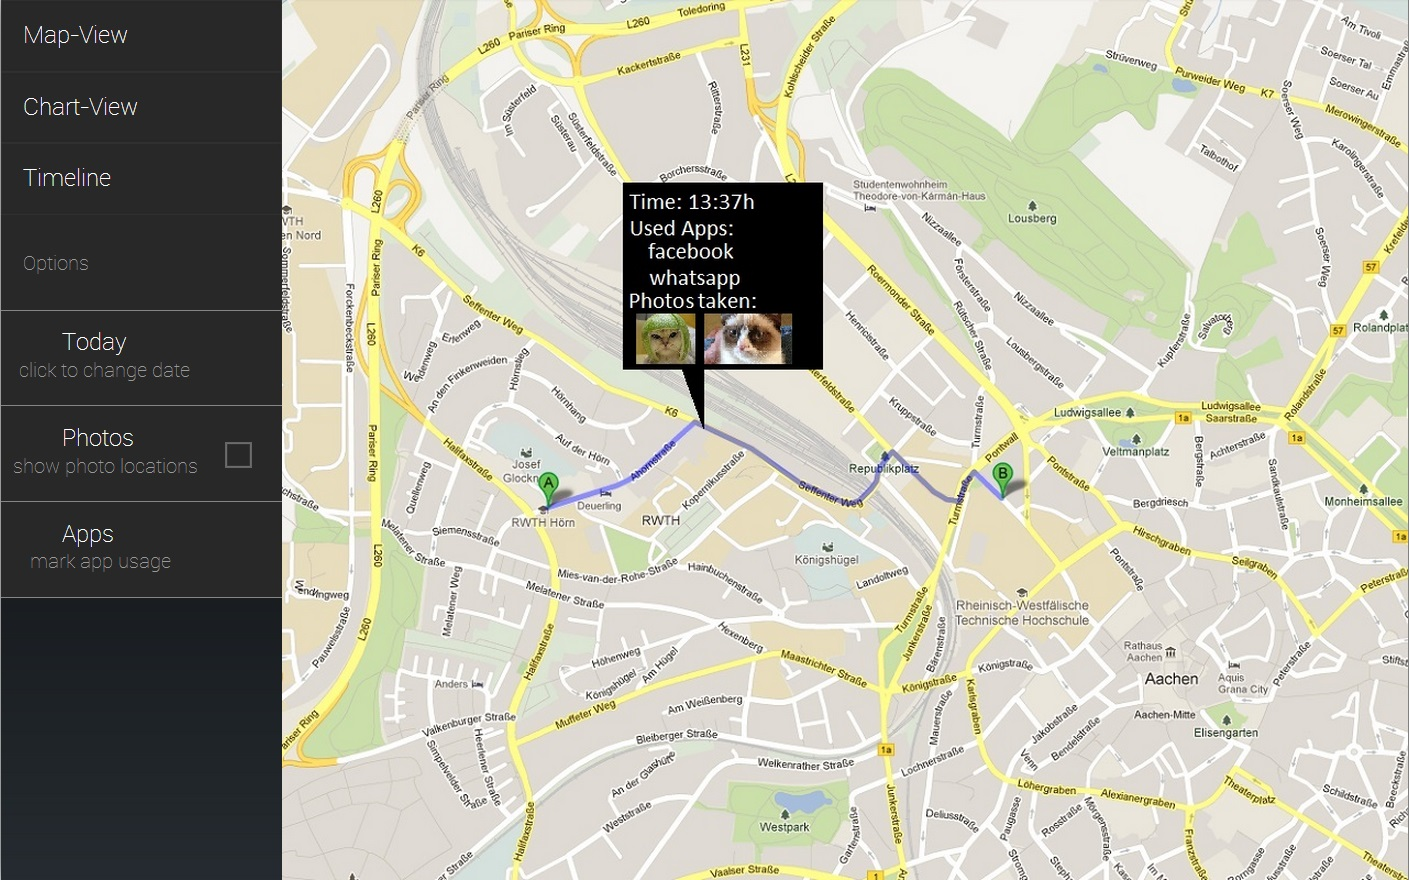
\includegraphics[width=\textwidth]{images/Design/1b_onClickPageView.jpg}
\end{figure}

The \mnote{Chart-View} second view, the chart view, shows the user his or hers daily activities in form of a pie chart. Its layout can be found in figure \ref{img:chartview}. The idea was to create location based charts that shows for each visited place the percentages of used applications. To break down the number of shown charts and thus to give a better overview, locations would be summarized in an intuitive way. That means that one has a chart for work, home and on the move. Those charts are lined up vertically and have an individual chart on the top of the list. This individual chart can be adjusted by the two extra options described in the following.\\
The \mnote{Chart-View specific options} first option lets one choose which places are taken into account for the individual chart. The second option determines which specific applications are displayed in the first chart. With these two options, one has the ability to to customize the first chart to visualize only those data which fit one's individual needs.

To \mnote{Grouping of apps and locations} get an even better overview, applications are classified into different groups. ``Social'' and ``Productive'' could be two groups, which split the applications apart. Applications like whatsapp and facebook may be social, while mail programs would be productive. The user would also be able to classify the applications by him- or herself, allowing to personalize the application. Furthermore, home, work and other places are chosen individually and extra places like parent's home can be added by the user, to give the him or her more space for customization.

To \mnote{Interacting with the view} get an better insight of the application groups, tapping on a slice of the pie chart will bring up a detailed view. In this detail view, one can see which applications are included in the tapped group and how large their percentage of daily activities is. In addition the total usage time of each application is shown, to give the displayed percentages more expressiveness.

The chart view, in contrast to the map view, is able to give a better overview over the percentages of used applications rather than show in which locations they have been utilized. It gives answer to the question ``What was the smartphone used for?''
\begin{figure}[h]
	\caption{Chart-View}
	\label{img:chartview}
	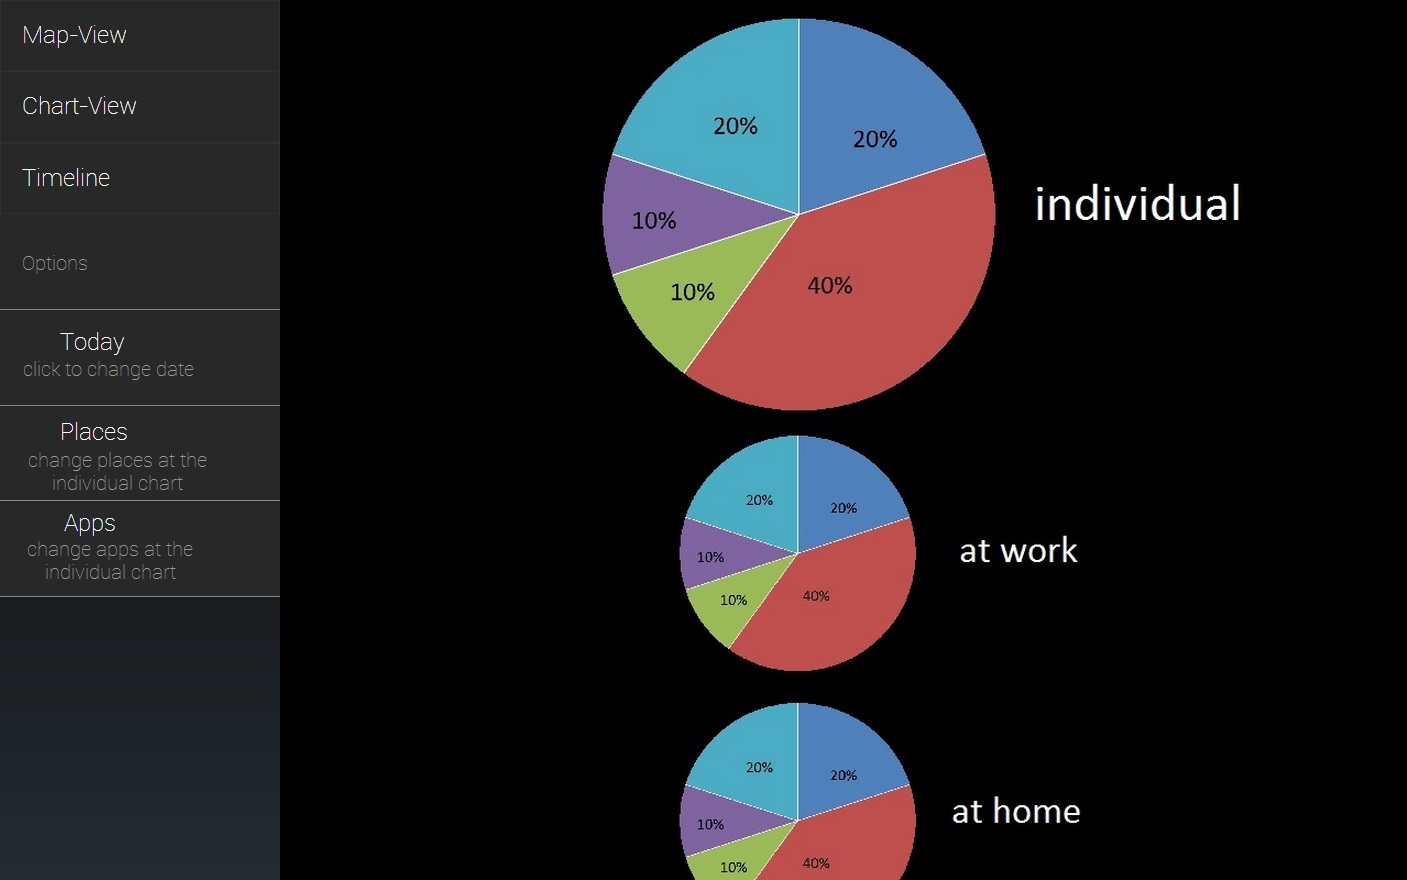
\includegraphics[width=\textwidth]{images/Design/2_ChartView.jpg}
\end{figure}

The \mnote{Timeline} timeline is the third and last view of this thesis' application. For a visual representation of the description of this view, please refer to figure \ref{img:timeline}. This view visualizes the daily activities in a chronological manner with two major parts. The first part is the the timeline itself and is described as follows. At the layout's bottom a horizontal line is draw with markings for every hour, from 0:00 to 24:00. Above this line, colored rectangles are drawn which represent a timespan in which an application was used. At the layout's top one can see markings for the visited location in dependence of the displayed timespan. One has the possibility to scroll horizontally through the view to observe the consecutively occur activities.

Beneath \mnote{The detailed view} the actual timeline a detailed view of all applications used on the selected date is found. This second part shows the application in descending order starting with the application mostly used on the chosen date. For each application a rectangle which represents the percentage of daily usage, is drawn. This rectangle will have the same color as the respective rectangles in the timeline and thus the detailed view can be used as a legend to identify the applications displayed in the timeline. Next to the application's bar the respective percentage and total amount of time is displayed.

This \mnote{Timeline specific options} view offers the extra option ``Apps'', where one can filter the displayed applications. With that option one is able to hide all other applications and display only those which are relevant for the user and thus giving the application a feel of personality and individuality.

Although it partially acts as a bar chart, the timeline, unlike the other views, focuses on the daily schedule by visualize the activities in a chronological order. With this view the user is able to answers the question ``When was the smartphone used?''.
\begin{figure}[h]
	\caption{Timeline}
	\label{img:timeline}
	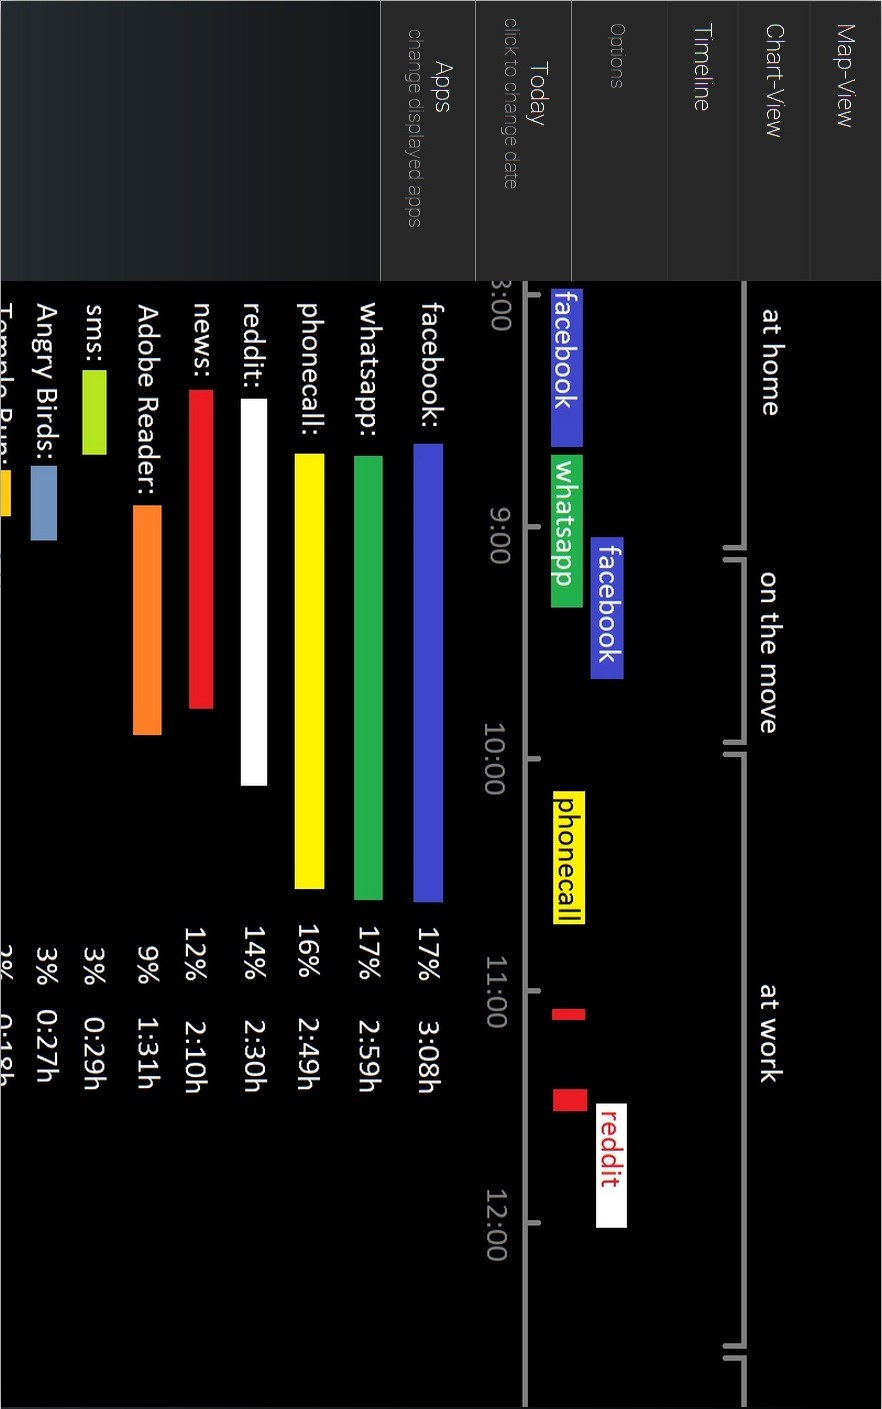
\includegraphics[width=\textwidth]{images/Design/3_TimeLine.jpg}
\end{figure}

As mentioned in the first place, this was the basic idea of the application and a few things have been changed during the development process. A summary of changes which differ from the paper prototype, along with the reasons for those changes can be found in the next sections.

%\newpage
%\section{Time Schedule}
%\label{subsec:time_schedule}
%For the proposal of this bachelor thesis a time schedule was created to structure the work flow. The estimated durations for each major task can be found in figure \ref{ganttchart1}.
%\begin{figure}[h]
%\begin{minipage}[][][c]{\textwidth}
%\caption{Gantt Chart: time schedule}
%\label{ganttchart1}
%\begin{ganttchart}{1}{17}
%	\gantttitle{Weeks}{17} \\
%	\gantttitlelist{1,...,17}{1} \\
%	\ganttbar{Research}{1}{2} \\
%	\ganttbar{Design Concept}{2}{4} \\
%	\ganttbar{Basic GUI}{3}{3} \\
%	\ganttbar{Chart View}{4}{5} \\
%	\ganttbar{Data Management}{6}{8}\\
%	\ganttbar{Timeline}{8}{9}\\
%	\ganttbar{Map View}{10}{11}\\
%	\ganttbar{Written Elaboration}{11}{17}
%\end{ganttchart}
%\end{minipage}
%\end{figure}
%
%The shown estimations were not always correct. The first weeks of this project went as planned and the incorporation in Android ran without greater problems. Likewise was the task of designing the paper prototype. In fact, the paper prototype took only one and a half weeks, therefore one had more time to focus on the basic user interface and the chart view.
%With start of the fifth week, the chart view was set up and first steps for data management were made. Unfortunately implementing the accessing of data, downloading, processing and storing took longer than expected, but the previously gained extra week could compensate it.\\
%The implementation of the timeline and the map view went as planned, but the writing of the written elaboration was not started until the 13. week due to polishing of visible and non visible parts of the application. Details about the progress of specific implementation parts are described in the next sections. 
\newpage
\section{Basic Layout}
The actual implementation work started with the creation of the basic layout. It characterizes the general picture of the application and has changed during the process of implementation.

%talk about lifecycle, provided views and viewgroups
When \mnote{View, Viewgroups and Fragments} the application first starts, one has to pass a layout to the main process, the main activity, to create a visible view. Those layouts are defined in xml and contain views and viewgroups. Basically, viewgroups contain views and/or other viewgroups and define their layout. For example one can define, whether visible views are ordered horizontally or vertically. Views contain the actual visible content, for instance a text or an image. Views are not static objects and can change during run time. One is also able to create and delete views and viewgroups during runtime, which will be helpful later. In order to create an application which looks and works like the paper prototype, one has to be able to change or switch whole groups of views in order to switch between map view, chart view and timeline. For this purpose one can use fragments.Fragments are kind of sub-activities which handle their own lifecycle and viewgroups and they are necessary for an interactive application, as they can be reused during runtime, thus provide an efficient way for switching views.

The first basic layout can be found in figure \ref{img:firstbasiclayout}. It resembles the paper prototype in functionality and appearance. Tapping on the view's name causes a view switch and options bring up pop up menus to select applications or a date.
To provide the application with the ability to react to user input, one can assign click listeners to views. After creating and assigning a click listener, Android calls it as soon as the user taps on an assigned view and a specified action, for instance a view switch, will be performed.
\begin{figure}[h]
	\caption{First Basic Layout}
	\label{img:firstbasiclayout}
	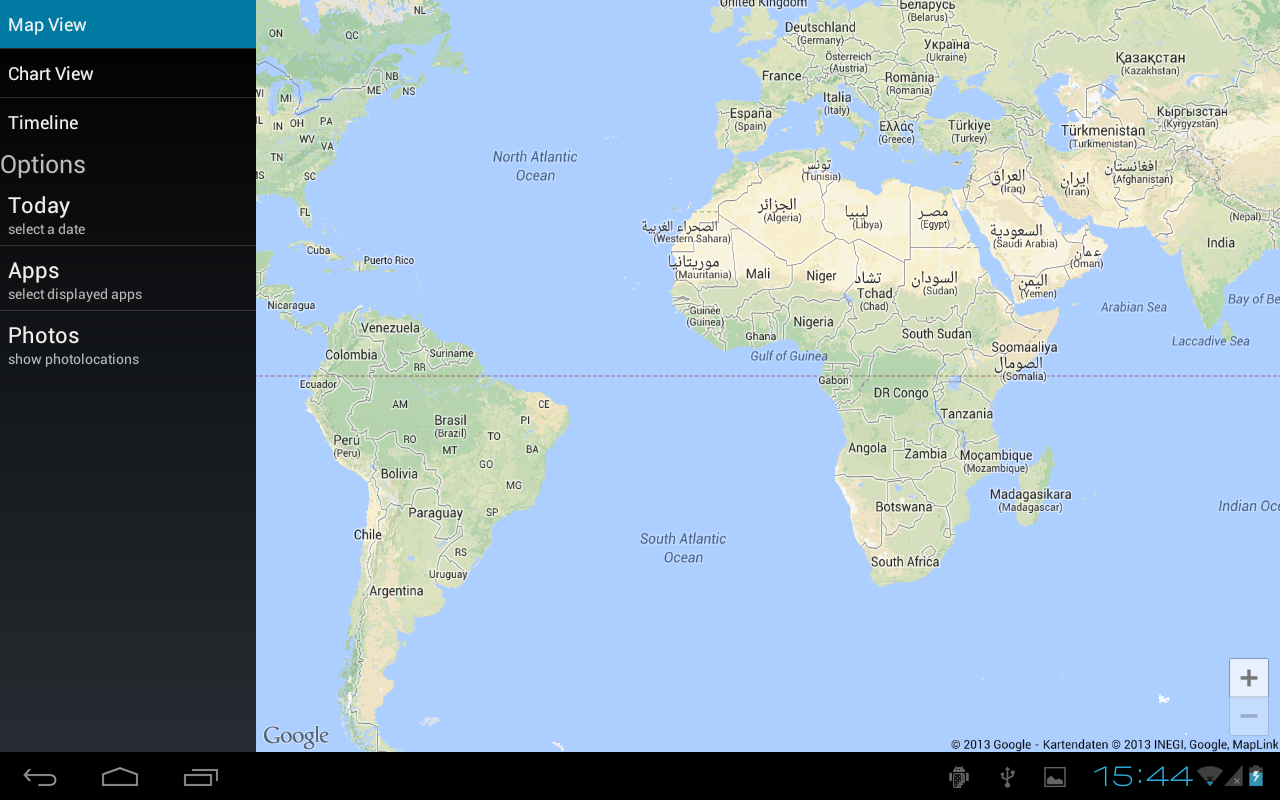
\includegraphics[width=\textwidth]{images/Screenshots/v3/Screenshot_2013-08-19-15-44-21.png}
\end{figure}

As \mnote{Visible fragments} mentioned above, at the start of the application the main activity needs a layout in order to create visible content. In this case the layout consists of three fragments. The first fragment is the view selection fragment. This is a list fragment which contains the three section names as views. The list fragment provides the programmer with the function \lstinline[language=Java]$onListItemClick$ which he or she can override. It gets called if one of the views names get clicked and is provided, among others, with the list position of the clicked view. With this information one is able to determine which view is requested and can then call the main activity to initiate a switch.\\
The second second fragment is the options fragment which is also a list fragment with the same abilities as the view selection fragment. If the user taps on an option the respective menu pops up and if the user makes adjustments the underlying dataset is updated and the main activity gets called to update the currently visible views.\\
The last fragment and most important in case of visualization and self reflection is the view section fragment. Those fragments visualize own layouts with different views which are described in their respective section.

In \mnote{Add and switch fragments} the first layout, the view selection fragment called the main activity in order to switch the view section fragment. To switch fragments the main activity uses the FragmentManager api. To obtain a FragmentManager object, the main activity calls \lstinline[language=Java]$getFragmentManager()$. With this object one can access a FragmentTransaction object, which is used to add or replace fragments. With the FragmentTransaction's function \lstinline$add(int, Fragment, String)$ one adds a fragment to a specific view. Do do so, one has to specify the container in which the fragment will be placed via an integer id previously assigned, the fragment to add to the container and an optional tag to access the fragment later. With a call of FragmentTransaction's function \lstinline$commit()$ the transaction will be executed.\\
To switch a fragment, one calls the FragmentTransaction's function \lstinline$replace(int, Fragment, String)$ with the same variables as previously described. It should be mentioned that only those fragments can be replaced that were added in a programmatically way and were not defined in the xml's layout file. Instead if just adding a new fragment to an occupied container one should use the \lstinline$replace()$ function or otherwise it can not be guaranteed that only one fragment is visible. But because \lstinline$replace()$ destroys the fragment, its rather inefficient if a user switches views very often, due to the fact that the fragment will be recreated every time it is added.\\
A solution to this problem are the FragmentTransaction's \lstinline$show()$ and \lstinline$hide()$ functions. These functions obviously show and hide fragments without destroying them, therefore they are more efficient in case of power consumption and calculation time. Another advantage is the maintaining of zoom and scroll positions without adding a single line of code.

To \mnote{Dialogs and DialogFragments} change the fragments appearance, one can tap on the options on the left side to bring up a pop up menu with a calendar or a checklist of application names. These option menus are created with Android's Dialog objects and controlled by the DialogFragment api. The first options menu, the calendar, is displayed by a special dialog, the DatePickerDialog which provides a visual appealing user interface to select a date. Once the option fragment created a DialogFragment, it has to assign itself as a listener to the object and call \lstinline$show()$ to Display the graphical user interface. To be able to handle the choice of a date, the DialogFragment implements DatePickerDialog's \lstinline$OnDateSetListener$, which gets called with the selected year, month and day if the user approves his or hers chosen date. Afterwards the DialogFragment calls the previous assigned listener and passes the the date to it. The options fragment then displays the selected date and stores it in the dataset, which notifies the main activity to update all visible fragments.\\
The other pop up options menu is also Dialog managed by a DialogFragment. It displays application names with a check box. To show this dialog, the options fragment creates a DialogFragment object and calls \lstinline$show()$. The options fragment does not have to assign itself as a listener but has to select a mode for the DialogFragment in order to load, display and store data correctly. Those modes are select\_apps, ignore\_apps and select\_highlight\_apps. Each mode builds its dialog identically with the help of a dialog builder. This builder offers different functions to create various dialogs and in this case is used to create a dialog with a multiple choice list and two buttons on the bottom. The builder provides a function called \lstinline$setMultiChoiceItems()$ with the following input variables. A string array of application names, an array of booleans representing checked states of the applications and a listener to handle click events. The application names and the boolean arrays are different for every mode, as they are loaded and gathered differently, for example the select\_apps mode only displays names of applications used at the currently selected date and forgets the selections after a restart, whereas the ignore\_apps mode loads all application names ever used by the owner an stores the selections in the dataset. The assigned listener tracks selection and deselection of list items and stores the application's name and the respective boolean for every change. If the user confirms his or hers selection, the dialog then stores according to the chosen mode, the selections in the dataset which again tells the main activity to update the fragments.

As \mnote{Change of the basic layout's visual appearance} the process of development progressed, the need of more options than previously assumed raised. Options for colorization of applications, switching the logged in user, deleting local files and permanently ignoring applications needed to be assigned to the layout. The problem with these options were, that they would not be used as much as selecting a date or temporarily hide displayed applications. Adding the options under the existing ones would cause a loss in simplicity and clarity of the application. The solution was Android's ActionBar api.

The ActionBar serves as a navigation bar which is set up at the top of the application and lets the programmer add tabs and option buttons, where option buttons can also be combined in small pop up menu. 
\begin{figure}[h]
	\caption{Final Basic Layout}
	\label{img:finalbasiclayout}
	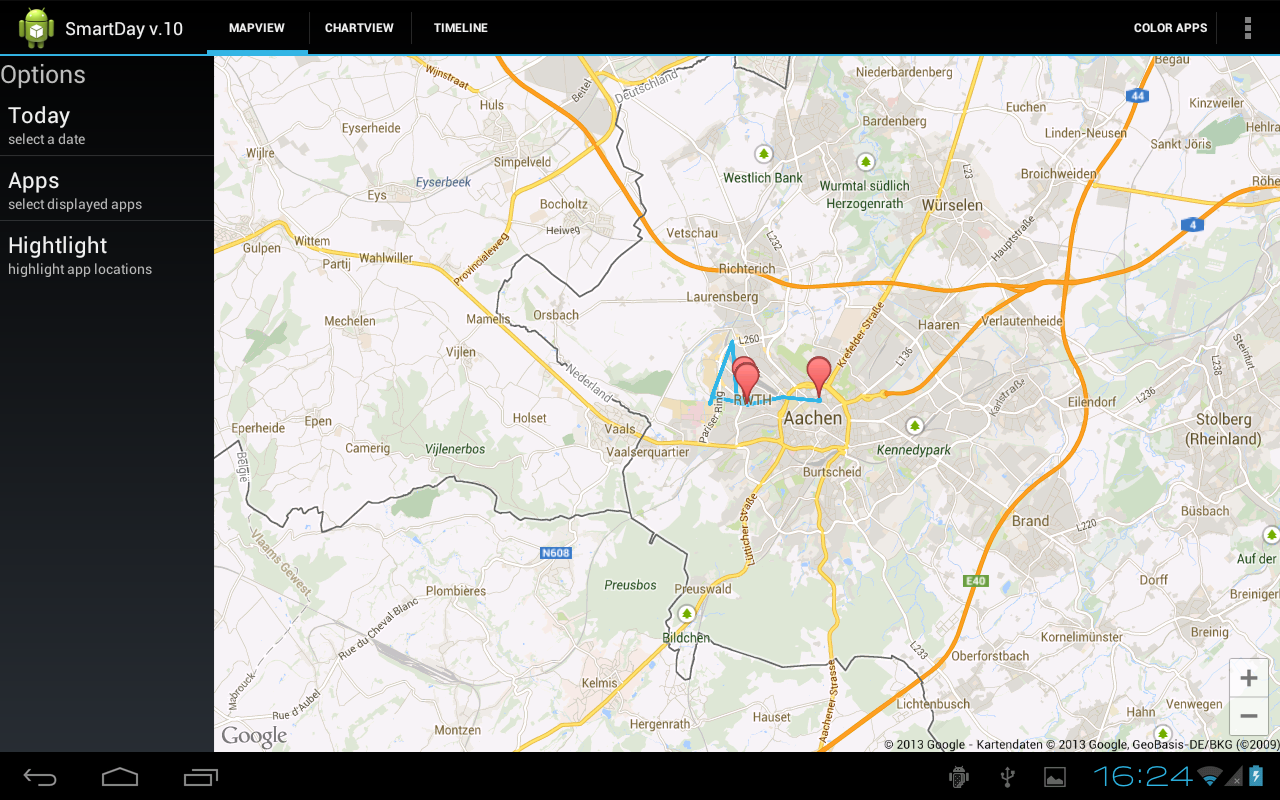
\includegraphics[width=\textwidth]{images/Screenshots/v10/Screenshot_2013-08-19-16-24-58.png}
\end{figure}

In \mnote{The action bar} order to make full use of the now used ActionBar, the former view selection fragment was deleted and the view's are now selected on the action bar by tapping on the new tab header. This layout is more intuitive as it resembles know patterns of Internet browsers and feels more structured. On the right side of the action bar, the color apps button is visible next to three dots which open a small list with the other new options - switch user, delete saved files and ignore apps. For more details see figure \ref{img:finalbasiclayout}.

The \mnote{Action bar tab header} main activity controls and sets up the bar as follows. By default, the action bar is visible in the application's layout but does not contain anything than the application's name in the top left corner. To add tab headers and options, one has to work with the ActionBar api. The main activity calls the function \lstinline$getActionBar()$, which returns an ActionBar object. With this object one can call the ActionBar's function \lstinline$newTab()$ to construct a new Tab object, which then has to be provided with a title via \lstinline$setText(String)$ and in order to react to taps, with a TabListener. In this thesis' application the TabListener class which implements the ActionBar's TabListener interface and manages its own tab and the respective fragment. The reference to the TabListeners are saved in the main activity, such that it can programmatically select or reselect a specific tab to notify changes or just to switch the tab. Once the data is provided, one can add the tabs to the ActionBar with a call of the ActionBar's function \lstinline$addTab(Tab)$.

Option buttons \mnote{Action bar option buttons} for the action bar are declared in an xml file. In this application the xml nodes representing the buttons by four key value pairs.
The first entry is an id, which is used to refer to the button from within the programs code. The title of the button is given in the field of the same name. A priority number to define the order of appearance of the buttons and an option to define if the button should be grouped under the three dots list or if it should directly be accessible on the action bar.\\
The main activity then has to override the function \lstinline$onOptionsItemSelcted()$ which gets the tapped button as input. With the previously assigned ids, one can differentiate between the four buttons and execute their respective functions which will be explained in the following.

The \mnote{Switch user} ``Switch User'' button allows the user to switch the profile accessing the visualized data. If this button is tapped, the main activity looks up if the user had stored his or her login information and deletes them. Then the underlying dataset function \lstinline$createNewUser()$ is called and the user is asked to provide new login data. The mentioned data set and its corresponding functions will be explained in section \ref{sec:datamanagement}.\\
``Delete Files'' \mnote{Delete files} gives the user the ability to regain occupied memory storage by deleting saved files. The main activity looks up the applications file directory and deletes any stored file, excluding the user login data. Those stored files are downloaded information about days along with colorings of displayed applications and the selection of ignored applications.\\
In \mnote{Ignore applications} order to permanently remove applications from selections and views, one can tap the ``Ignore Apps'' button. This causes the main application to request every used application from the dataset by calling \lstinline$getAllApps()$. After the dataset has downloaded all application names from the server, the main activity creates a dialog where the user can pick applications which will be hidden permanently. The selection will then be stored in the dataset and all views will be updated.\\
The \mnote{Color apps} button which is visible as long as the screen sizes offers enough space, is the ``Color Apps'' button. Tapping this button causes the main activity to create a dialog displaying application names with respectively colored rectangles next to them. A tap on the application name or rectangle unveils a new pop up menu which lets the user pick a color as seen in figure \ref{img:colorpicker}.
\begin{figure}[h]
	\caption{Color picker}
	\label{img:colorpicker}
	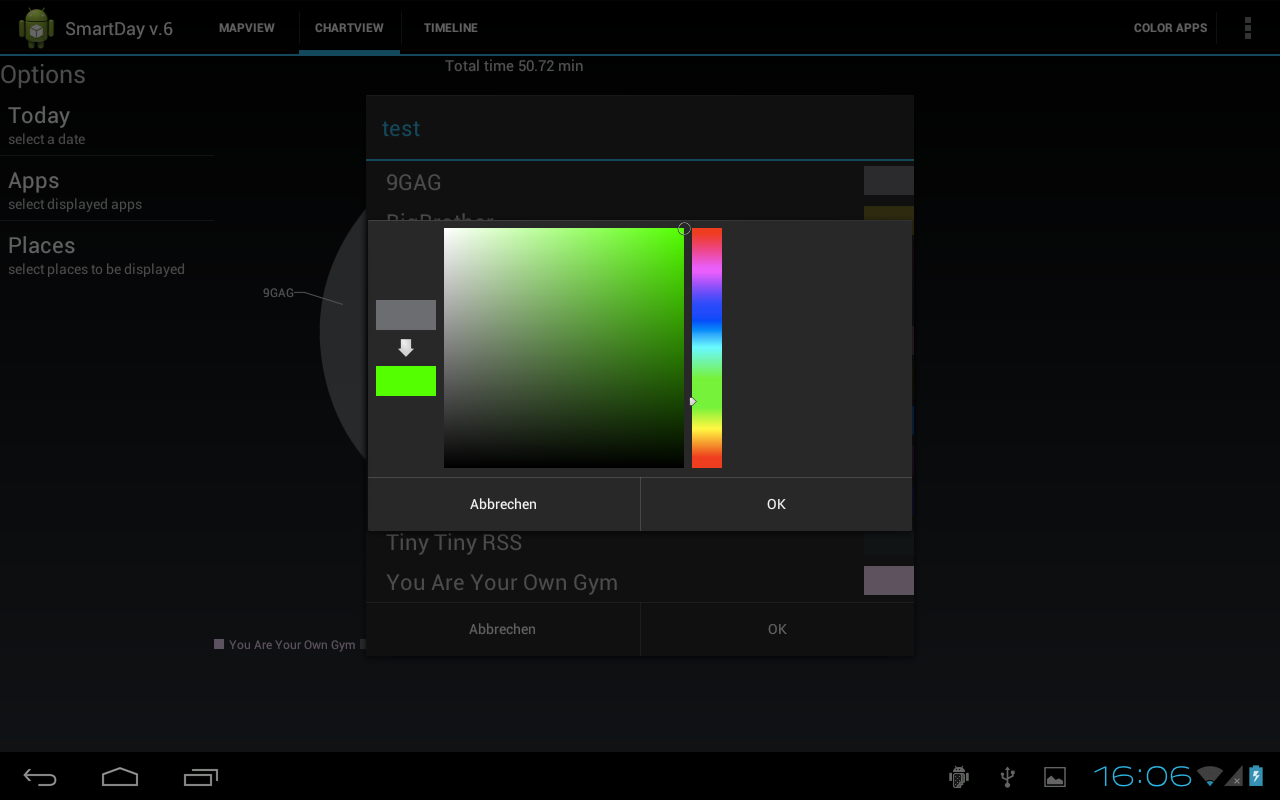
\includegraphics[width=\textwidth]{images/Screenshots/v6/Screenshot_2013-08-19-16-06-13.png}
\end{figure}

This new pop up is built with Yuku Sugianto's Android Color Picker or the Indonesian translation Ambil Warna\cite{colorpicker}. To use this color picker, one has to include the source code into its own application code and define it as a library project in order to access functions and classes. Once the Ambil Warna was linked as a library project, the application uses it as follows. As soon as an application name or the respective rectangle is tapped, the \lstinline$onClickListener$ extracts its own title, which is the applications name and creates an \lstinline$OnAmbilWarnaListener$ which overwrites the functions \lstinline$onOk()$ and \lstinline$onCancel()$ which are listeners and get called if their respective button is tapped. If \lstinline$onOk()$ is called, the function stores the color and respective application name and afterwards updates the color of the rectangle.\\
After \mnote{The AmbilWarnaDialog} the construction of the \lstinline$OnAmbilWarnaListener$, the \lstinline$AmbilWarnaDialog$ will be created by passing the current activity, the start color and the listener. With a call of \lstinline$show()$ the dialog is displayed and the user can interact with it. Once the user has picked all colors and hits ok, the dialog stores the new colors in the data set which then notifies the main activity to update its fragments. If the user decides that he or she does not want to apply the changes and taps cancel, all changes are discarded.

The basic layout is an essential part of the application experience. It offers not only a structured layout for view corresponding options and general ones, but it also presents a surrounding structure for views themselves. The possibility to seamlessly attach new views with tab headers and options on the left option fragment without destroying the uniform appearance of the application may be an advantage for possible future projects.\\
The basic layout was created to be minimal in terms of displayed options in order to prevent distraction from the actual function of this application, the self reflection.
\newpage
\section{Data Management}
\label{sec:datamanagement}
In the last section the term of a data set was mentioned a few times. This data set or the managing class of it will be explained in this section. It is the essential for the whole application, as it provides every fragment with the needed user data. The construction of this class was one of the hardest part of developing SmartDay and pieces of it were rewritten or removed as the development of the different fragments proceeded. Especially notifications for the main activity in order to update views if new data was available have been adjusted a few times.

The \mnote{JSON format} application's underlying dataset is stored in a \emph{JavScript Object Notation}, in short JSON, format. JSON structures consist of  key:value pairs, where the value can be a number, string, object or array. Keys and strings are enclosed by quotation marks and the key is separated from the value by a colon. An object is enclosed by curly braces and contains a collection of key:value pairs, each separated with a comma. An array is a collection of objects, each separated by a comma and enclosed by square brackets. JSON offered an easy way to handle the data provided by the server and was also natively supported by Android. The following sample describes the actual structure of the JSON object which is primarily used by the application and can be seen in figure \ref{fig:jsonobject}.
\begin{figure}
\caption{The Basic JSON Object}
\label{fig:jsonobject}
\begin{lstlisting}[language=json,firstnumber=1]
{ "dateTimestamp": long,
  "downloadTimestamp": long,
  "totalDuration": long,
  "result":[
    { "app": string,
      "duration": long,
      "usage":[
          { "session": string,
            "start": long,
            "end": long,
            "location":[
                 {"key": "lat",
                  "value": long
                 },
                 {"key": "lng",
                  "value": long
                 }
            ]}, ...
      ]}, ...
  ]
}
\end{lstlisting}
\end{figure}

In \mnote{JSON object in SmartDay} the top level object, the structure holds informations about download and date time stamp, along with the total time of application usages. In this application, all information about time are given in seconds precision. The JSON object holds an array called result and contains a JSON object for every application used at the specific day. Each of these objects contains a field app with the application's name stored as a string and a field duration, containing the total duration time of the application. Each object also contains an array \emph{usage}. This array contains objects of every timespan in which the application was used. Every usage object contains keys start and end with respective time stamps for start and end time. In addition the field session contains the applications session id and an array \emph{location} is given which contains two objects. These objects contain a key:value pair key which identifies whether the object holds information about the longitude or latitude, by storing a string with content lng respectively lat. The actual position information is stored in the value field which stores it as double.\\
With these information one has all needed data to create the fragments reflecting one's daily activities.

The \mnote{DataSet initialization} data managing class \emph{DataSet} is designed to be a singleton to guarantee that every view and fragment of the application is provided with the same data. In order to obtain a \lstinline$DataSet$ instance, one can call \lstinline$getInstance()$ which returns an instance of \lstinline$DataSet$ or initializes one and returns it, if none exists. In the process of initialization, the instance requests a new object of the class \lstinline$UserData$ which holds the user name and password. While the \lstinline$UserData$ object is created, it is directly checked, if the data is correct by contacting the server, but this will be explained later in this section. After requesting user data, it is checked, whether data for colorization and for ignoring applications are stored locally and can be loaded or not. If files are available, they are read and respective JSON objects are created and stored. After \lstinline$UserData$ calls \lstinline$DataSet$ to pass a successfully created and tested user object it is stored and the date is initialized. Since the application provides support to display data of multiple days in one fragment, the current date is determined, stored and selected as start and end date, meaning that at the time of initialization only one date, the current day is selected. Storing of the current date is only necessary to check if a chosen date equals the current date and thus label it as ``Today''.\\
Once the initialization part and therefore the creation of the \lstinline$DataSet$ instance is completed, the instance calls its own function \lstinline$getApps(Listener)$ with \lstinline$null$ as listener. This function requests a download of data of the selected day and the reason for the call with \lstinline$null$ is, that in this way the main activity is notified that the data is available for first time and it can set up the fragments for the first time which need the data.

As mentioned, \mnote{Creating a new user} the a new user object is requested from \lstinline$UserData$. This is done by calling \lstinline$getUserLoginData$. This function is provided with the main activity and an optional boolean as parameters. The main activity is needed to for different functionalities like storing data in a local file or accessing the Internet, which is explained later. The boolean can be set to true if one wants to create a new user, ignoring and deleting stored user files. This is needed if one wants to switch the user login data the application uses. In case no stored user data is available, the application shows a dialog in which one can type in user name and password. In addition, one can check a box to tell the application, that his or her should be saved. Once the user hits ok, the data will be stored according to the check box and then the login data will be tested. If the server's reply to the test is positive the user data is passed to the \lstinline$DataSet$, else the dialog is shown again.

To \mnote{Asynchronous tasks} communicate with a server one has to note a few things. First, the communication has to be executed on a separate thread. One does not want the main thread to handle the download because waiting for a server response may occupy the thread for a few seconds and thus other actions are not possible during this time. And due to the use of an asynchronous thread one should ensure that at some point the downloaded data gets passed to the requester in order to be able to display the data.\\
Android provides a good solution to handle short usages of asynchronous tasks. The \lstinline$AsyncTask$ api offers the ability to easily create and maintain a separate thread. To use its functionality, one has to extend \lstinline$AsyncTask<Params,Progress,Result>$, define the three generic types and overwrite the following functions.\lstinline$onPreExecute$ gets called on the main thread and is used in this application to bring up an dialog, showing that something like the testing of user data is done right at the moment.  \lstinline$doInBackground$ is the actual function which runs on the new thread. It gets Params as input and returns Result. In this application the server access and the downloading of data are implemented into this function. The last function\lstinline$onPostExecute$ is called after the asynchronous tasks is finished. It is used to remove the dialog which was set up in \lstinline$onPreExecute$ and processes Result which was returned by \lstinline$doInBackground$.\\
Once the class has been implemented, one can instantiating it and then call \lstinline$execute(Params)$ to execute the asynchronous task.

Now \mnote{Server access} the use of asynchronous tasks has been clarified, 

\newpage
\section{Mapview}

\newpage
\section{Chartview}

\newpage
\section{Timeline}

